\documentclass{article}
\usepackage[a4paper]{geometry}
\usepackage[brazil]{babel}
\usepackage[utf8]{inputenc}
\usepackage{url}
\usepackage{hyperref}
\usepackage{graphicx}
\usepackage{amsmath}
\usepackage{amsfonts}
\usepackage{amssymb}

\title{Atividade 3 - Técnica de Relaxação Lagrangiana para o kSTSP}
\author{
	Lucas Guesser Targino da Silva - RA: 203534 \\
    Renan Fernando Franco da Silva - RA: 223989
}

\newcommand{\secref}[1]{(Seção \ref{#1})}
\newcommand{\subsecref}[1]{(Subseção \ref{#1})}
\newcommand{\constraintRef}[1]{Restrição \ref{#1}}
\newcommand{\figref}[1]{Figura \ref{#1}}

\newcommand{\Set}[1]{\ensuremath{\left\{#1\right\}}}
\newcommand{\partsof}[1]{\ensuremath{\mathcal{P}\left(#1\right)}}
\newcommand{\Sum}[1]{\ensuremath{\displaystyle\sum\limits_{#1}}}
\newcommand{\abs}[1]{\ensuremath{\left| #1 \right|}}
\newcommand{\binary}{\ensuremath{\Set{0, 1}}}

\newcommand{\edge}{\ensuremath{e}}
\newcommand{\edges}{\ensuremath{E}}
\newcommand{\vertex}{\ensuremath{v}}
\newcommand{\vertices}{\ensuremath{V}}
\newcommand{\nvertices}{\ensuremath{\abs{\vertices}}}
\newcommand{\ncycles}{2}
\newcommand{\allCycles}{\ensuremath{\Set{1, \ncycles}}}
\newcommand{\cycle}{\ensuremath{k}}
\newcommand{\subvertices}{\ensuremath{S}}
\newcommand{\graph}{\ensuremath{G}}
\newcommand{\cost}[1]{\ensuremath{c^{#1}}}
\newcommand{\costk}{\ensuremath{\cost{\cycle}}}
\newcommand{\costke}{\ensuremath{\cost{\cycle}_{\edge}}}
\newcommand{\co}[1]{\ensuremath{c^{1}}}
\newcommand{\ct}{\ensuremath{c^{2}}}
\newcommand{\coe}{\ensuremath{c^{1}_{\edge}}}
\newcommand{\cte}{\ensuremath{c^{2}_{\edge}}}
\newcommand{\positiveReal}{\ensuremath{\mathbb{R}_+}}
\newcommand{\X}[2]{\ensuremath{x^{#1}_{#2}}}
\newcommand{\xke}{\ensuremath{\X{\cycle}{\edge}}}
\newcommand{\xoe}{\ensuremath{x^{1}_{\edge}}}
\newcommand{\xte}{\ensuremath{x^{2}_{\edge}}}
\newcommand{\ze}{\ensuremath{z_{\edge}}}
\newcommand{\similarity}{\ensuremath{\sigma}}
\newcommand{\totalconstraints}{\ensuremath{T_r}}
\newcommand{\bigo}[1]{\ensuremath{\mathcal{O}\left( #1 \right)}}

\newcommand{\lagrange}{\ensuremath{\lambda}}
\newcommand{\lagrangeke}{\ensuremath{\lagrange_{\edge}^{\cycle}}}

\begin{document}

\maketitle

\section{Enunciado do Problema}

Sejam:

\begin{enumerate}
    \item $\graph = \langle \vertices,\edges \rangle$: um grafo não-orientado completo:
    \begin{enumerate}
        \item $\vertices$: conjunto de vértices;
        \item $\edges$: conjunto das arestas;
    \end{enumerate}
    \item $\costk: \edges \rightarrow \positiveReal,\ \forall \cycle \in \allCycles$, duas funções custo nos vértices;
        \begin{enumerate}
            \item dada uma aresta $\edge$, escrevemos $\costk(\edge) = \costke$;
        \end{enumerate}
    \item $\similarity$: parâmetro de similaridade de ciclos;
\end{enumerate}

Objetivo: encontrar dois ciclos Hamiltonianos com custo total mínimo, tal que pelo menos $\similarity$ arestas do grafo sejam visitadas por ambos os ciclos.

\section{Modelo Matemático}
\label{sec:mathematical model}

Nessa seção, será apresentada a formulação do problema utilizando Programação Linear Inteira. Esse não foi resolvido diretamente (j[a que não é o intuito da atividade), mas foi utilizado para derivar uma Relaxação Lagrangiana \secref{sec:lagrangian relaxation}, que foi modelo de fato implementado e resolvido.

\subsection{Variáveis de Decisão}
\label{constraint:variables}

\begin{itemize}
	\item $\xke$: presença da aresta $\edge$ no ciclo $\cycle$;
	\item $\ze$: presença de duplicação da aresta $\edge$;
\end{itemize}

Todas as variáveis de ``presença'' são decisões binárias com a seguinte interpretação de valores:

\begin{itemize}
	\item[0]: ausente
	\item[1]: presente
\end{itemize}

\subsection{Problema de Otimização}
\label{subsec:problem}

Minimizar:
\begin{equation}
    \label{eq:goal}
 	\Sum{\cycle \in \allCycles}
 	\Sum{\edge \in \edges} 	
 	\costke \ \xke 	
\end{equation}

Sujeito a:
\begin{equation}
	\label{constraint:vertex presence}
	\Sum{\edge \in \delta(\vertex)} \xke = 2
	\qquad
	\forall \vertex \in \vertices,
	\forall \cycle \in \allCycles
\end{equation}

\begin{equation}
	\label{constraint:no subcycle}
	\Sum{\edge \in \edges(\subvertices)} \xke \leqslant \abs{\subvertices} - 1
	\qquad
	\forall
		\subvertices \subseteq \vertices,
		\subvertices \neq \vertices,
		\subvertices \neq \emptyset,
		\forall \cycle \in \allCycles
\end{equation}

\begin{equation}
	\label{constraint:similarity compatibility}
	\xke \geqslant \ze
	\qquad
	\forall \edge \in \edges,
	\forall \cycle \in \allCycles
\end{equation}

\begin{equation}
	\label{constraint:similarity}
	\Sum{\edge \in \edges} \ze \geqslant \similarity
\end{equation}

\begin{equation}
	\label{constraint:binary variables}
	\xke, \ze \in \binary
	\qquad
	\forall \edge \in \edges,
	\forall \cycle \in \allCycles
\end{equation}

\subsection{Explicação das Restrições}
\label{subsec: constraints explanation}

\begin{itemize}
    \item A função objetivo \eqref{eq:goal} é soma do custo de todas as arestas selecionadas em todos os ciclos.
    \item A restrição \eqref{constraint:vertex presence} garante que a quantidade de arestas incidentes em todos os vértices seja 2. Essa condição faz com que todos os vértices tenham que ser visitados (duas arestas pois uma é a de ``entrada'' e a outra a de ``saída'').
    \item A restrição \eqref{constraint:no subcycle} garante que não existam subciclos nos ciclos. Nessa restrição, $\subvertices$ é um subconjunto próprio e não-vazio dos vértices do problema. A expressão $\edges(\subvertices)$ é o conjunto das arestas cujos vértices (ambos) estão em $\subvertices$.
    \item A restrição \eqref{constraint:similarity compatibility} garante que, se uma aresta foi escolhida para ser duplicada, então essa aresta aparecerá nos dois ciclos.
    \item A restrição \eqref{constraint:similarity} garante que pelo menos $\similarity$ arestas serão escolhidas para serem duplicadas.
    \item A restrição \eqref{constraint:binary variables} garante que todas as variáveis são decisões binárias, ou seja, assumem apenas um de dois possíveis valores: 0 e 1.
\end{itemize}

\subsection{Tamanho das Restrições}
\label{subsec:constraints size}

\begin{itemize}
	\item Restrição \eqref{constraint:vertex presence}: uma para cada vértice e para cada ciclo. Total: $\ncycles \cdot \abs{\vertices}$;
	\item Restrição \eqref{constraint:no subcycle}: uma para $\subvertices \in \partsof{\vertices}, \subvertices \neq \vertices, \subvertices \neq \emptyset$ e para cada ciclo. Total: $\ncycles \cdot \left( 2^{\abs{\vertices}} - 2\right)$;
	\item Restrições \eqref{constraint:similarity compatibility}: uma para cada aresta e para cada ciclo. Total: $\ncycles \cdot \abs{\edges} = \ncycles \cdot \dfrac{\abs{\vertices}^2 - \abs{\vertices}}{2}$ (já que o grafo é completo);
	\item Restrições \ref{constraint:similarity}: apenas uma. Total: 1;
\end{itemize}

Assim, o número total de restrições é:

\begin{equation}
	\totalconstraints =
		  \ncycles \cdot \abs{\vertices}
		+ \ncycles \cdot \left( 2^{\abs{\vertices}} - 2\right)
		+ \ncycles \cdot \dfrac{\abs{\vertices}^2 - \abs{\vertices}}{2}
		+ 1
\end{equation}

Assim:

\begin{equation}
	\label{eq:number of constraints}
	\totalconstraints \in \bigo{2^{\nvertices}}
\end{equation}

Note que há um número exponencial de restrições.

% Na implementação computacional do problema, não é possível adicionar tantas restrições por falta de recursos computacionais (memória e processamento). Há entretanto uma forma de contornar o problema atŕavés do que se chama de \textit{lazy evaluation}. A ideia é não adicionar tais restrições no início. Conforme soluções factíveis são encontradas, verifica-se se há subciclos nelas e, caso sim, adiciona-se apenas as restrições necessárias para eliminar tais subciclos.
%
% Dependendo do caso em mãos, essa abordagem pode reduzir drasticamente o número de restrições e consequentemente acelerar a busca.

\section{Relaxação Lagrangiana}
\label{sec:lagrangian relaxation}

\subsection{Escolha da Restrição a ser Relaxada}

A técnica de Relaxação Lagrangiana consiste em escolher uma ou mais restrições para relaxar. Tal escolha visa remover as restrições que fazem do problem ``difícil de ser resolvido'' \cite{bib:linear-optimization-intro}.

\subsubsection{Análise das Restrições}

\begin{itemize}
	\item \constraintRef{constraint:vertex presence}: não parece ser uma restrição difícil;
	\item \constraintRef{constraint:no subcycle}: essa restrição é de fato difícil. Entretanto, há um número exponencial delas, de forma que é inviável relaxá-la. Além disso, há técnicas que lidam bem com ela\footnote{\textit{Lazy constraints} por exemplo, abordado no trabalho anterior.};
	\item \constraintRef{constraint:similarity compatibility}: no trabalho anterior, notou-se que o fator de similaridade causa bastante impacto no tempo computacional \figref{figure:previous running time}. Isso significa que ele deixa o problema difícil, sendo então um bom candidato à relaxação;
	\item \constraintRef{constraint:similarity}: essa restrição tem efeitos bem parecidos com a \constraintRef{constraint:similarity compatibility}. Ela representa, entretanto, apenas uma equação de restrição, não sendo assim interessante para a relaxação;
	\item \constraintRef{constraint:binary variables}: já é considerada a relaxação dessa restrição pelo método;
\end{itemize}

Portanto, a restrição escolhida para ser relaxada é a \constraintRef{constraint:similarity compatibility}.

\begin{figure}
    \centering
    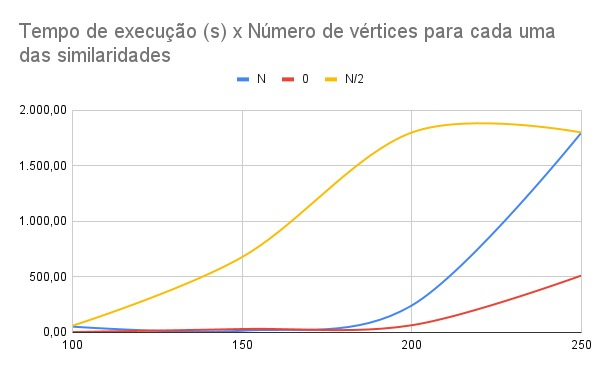
\includegraphics[width=0.7\textwidth]{images/running_time.jpeg}
    \caption{tempo de execução dos experimentos do trabalho anterior.}
    \label{figure:previous running time}
\end{figure}

\subsection{Modelo Matemático da Relaxação Lagrangiana}
\label{subsec:lagrangian relaxation}

Minimizar:
\begin{equation}
    \label{eq:goal lagrangian}
 	\Sum{\cycle \in \allCycles}
 	\Sum{\edge \in \edges} 	
 	\costke \ \xke
 	+ \lagrangeke \left( \ze - \xke \right)
\end{equation}

Sujeito às restrições \ref{constraint:vertex presence}, \ref{constraint:no subcycle}, e \ref{constraint:similarity} do problema original \subsecref{subsec:problem}, e a restrições de domínio:

\begin{equation}
	\label{constraint:value of variables}
	0 \leqslant \xke, \ze \leqslant 1
	\qquad
	\forall \edge \in \edges,
	\forall \cycle \in \allCycles
\end{equation}

\begin{equation}
	\label{constraint: lagrange}
	\lagrangeke \geqslant 0
	\qquad
	\forall \edge \in \edges,
	\forall \cycle \in \allCycles
\end{equation}

\subsection{Método do Subgradiente}

{\huge TO DO}

Descrever como fazemos para atualizar $\lagrangeke$.

\subsection{Heurística Lagrangiana}

{\huge TO DO}

Descrever como transformamos uma solução infactível numa solução factível.

\section{Algoritmo de Solução do Problema}

{\huge TO DO}

Descrever o algoritmo completo, em pseudocódigo.

\section{Experimento Computacional}

\subsection{Configuração da Máquina}

O problema foi executado num ideapad S145 81S90005BR: Lenovo IdeaPad S145 Notebook Intel Core i5-8265U (6MB Cache, 1.6GHz, 8 cores), 8GB DDR4-SDRAM, 460 GB SSD, Intel UHD Graphics 620.

O sistema operacional foi o Fedora 35 executando gcc (GCC) 11.2.1 20220127 (Red Hat 11.2.1-9), Concorde \cite{bib:concorde} e o solver QSOpt \cite{bib:qsopt}.

Como linguagem de programação, utilizamos C++ \cite{bib:cpp}.


\subsection{Dados do Problema}

Os dados do problema foram fornecidos em um arquivo contendo 4 colunas e 250 linhas. A interpretação dos dados é a seguinte: cada linha representa um vértice e cada par de coluna as coordenadas desse vértice. A razão para um vértice ter duas posições diferentes é simplesmente para que as distâncias entre eles tenham valores diferentes no primeiro e no segundo ciclo.

O modelo na verdade precisa apenas de pesos. Construímos a primeira função de custo como a distância euclidiana entre os pontos das colunas 1 e 2. Da mesma forma, utilizamos distância euclidiana entre os pontos das colunas 3 e 4 para construir a segunda função de custo.

Note que, com essa interpretação, parece que temos dois conjuntos de vértices, um definido pelas colunas 1 e 2, e outro definido pelas colunas 3 e 4. Conforme explicitado no primeiro parágrafo da seção, esse não é o caso. Cada linha é um vértice e os valores fornecidos servem apenas para calcular a distância euclidiana e usá-la como peso para as arestas. Dessa forma, a aresta que liga os vértices representados pelas linhas 12 e 84, por exemplo, possui dois pesos diferentes, um para ser utilizado no primeiro ciclo e outro para ser utilizado no segundo.

\subsection{Geração das Instâncias}

Para gerar instâncias de um dado tamanho $N$, utilizamos as primeiras $N$ linhas dos dados fornecidos.

\subsection{Resultados}

{\huge TO DO}

\subsection{Análise dos Resultados}

{\huge TO DO}

\bibliographystyle{ieeetr}
\bibliography{bibliography}

\end{document}
